
%%%%%%%%%%%%%%%%%%%%%%%%%%%%%%%%%%%%%%%%%%%%%%%%%%%%%%%%%%%%%%%%%%%%%%%%%%%%%%%%%%%%%%%
%%%%%%%%%%%%%%%%%%%%%%%%%%%%%%%%%%%%%%%%%%%%%%%%%%%%%%%%%%%%%%%%%%%%%%%%%%%%%%%%%%%%%%%
% 
% This top part of the document is called the 'preamble'.  Modify it with caution!
%
% The real document starts below where it says 'The main document starts here'.

\documentclass[12pt]{article}

\usepackage{amssymb,amsmath,amsthm}
\usepackage[top=1in, bottom=1in, left=1.25in, right=1.25in]{geometry}
\usepackage{fancyhdr}
\usepackage{enumerate}
\usepackage{listings}
\usepackage{graphicx}
\usepackage{float}
\usepackage{amsmath}
% Comment the following line to use TeX's default font of Computer Modern.

\usepackage{times,txfonts}



\makeatletter
\renewcommand*\env@matrix[1][*\c@MaxMatrixCols c]{%
  \hskip -\arraycolsep
  \let\@ifnextchar\new@ifnextchar
  \array{#1}}
\makeatother

\newtheoremstyle{homework}% name of the style to be used
  {18pt}% measure of space to leave above the theorem. E.g.: 3pt
  {12pt}% measure of space to leave below the theorem. E.g.: 3pt
  {}% name of font to use in the body of the theorem
  {}% measure of space to indent
  {\bfseries}% name of head font
  {:}% punctuation between head and body
  {2ex}% space after theorem head; " " = normal interword space
  {}% Manually specify head
\theoremstyle{homework} 

% Set up an Exercise environment and a Solution label.
\newtheorem*{exercisecore}{Exercise \@currentlabel}
\newenvironment{exercise}[1]
{\def\@currentlabel{#1}\exercisecore}
{\endexercisecore}

\newcommand{\localhead}[1]{\par\smallskip\noindent\textbf{#1}\nobreak\\}%
\newcommand\solution{\localhead{Solution:}}

%%%%%%%%%%%%%%%%%%%%%%%%%%%%%%%%%%%%%%%%%%%%%%%%%%%%%%%%%%%%%%%%%%%%%%%%
%
% Stuff for getting the name/document date/title across the header
\makeatletter
\RequirePackage{fancyhdr}
\pagestyle{fancy}
\fancyfoot[C]{\ifnum \value{page} > 1\relax\thepage\fi}
\fancyhead[L]{\ifx\@doclabel\@empty\else\@doclabel\fi}
\fancyhead[C]{\ifx\@docdate\@empty\else\@docdate\fi}
\fancyhead[R]{\ifx\@docauthor\@empty\else\@docauthor\fi}
\headheight 15pt

\def\doclabel#1{\gdef\@doclabel{#1}}
\doclabel{Use {\tt\textbackslash doclabel\{MY LABEL\}}.}
\def\docdate#1{\gdef\@docdate{#1}}
\docdate{Use {\tt\textbackslash docdate\{MY DATE\}}.}
\def\docauthor#1{\gdef\@docauthor{#1}}
\docauthor{Use {\tt\textbackslash docauthor\{MY NAME\}}.}
\makeatother

% Shortcuts for blackboard bold number sets (reals, integers, etc.)
\newcommand{\Reals}{\ensuremath{\mathbb R}}
\newcommand{\Nats}{\ensuremath{\mathbb N}}
\newcommand{\Ints}{\ensuremath{\mathbb Z}}
\newcommand{\Rats}{\ensuremath{\mathbb Q}}
\newcommand{\Cplx}{\ensuremath{\mathbb C}}
%% Some equivalents that some people may prefer.
\let\RR\Reals
\let\NN\Nats
\let\II\Ints
\let\CC\Cplx

%%%%%%%%%%%%%%%%%%%%%%%%%%%%%%%%%%%%%%%%%%%%%%%%%%%%%%%%%%%%%%%%%%%%%%%%%%%%%%%%%%%%%%%
%%%%%%%%%%%%%%%%%%%%%%%%%%%%%%%%%%%%%%%%%%%%%%%%%%%%%%%%%%%%%%%%%%%%%%%%%%%%%%%%%%%%%%%
% 
% The main document start here.

% The following commands set up the material that appears in the header.
\doclabel{STAT 402: Homework 6}
\docauthor{Stefano Fochesatto}
\docdate{October 15, 1021}


%\textbf{Code:}
%\begin{center}
 %   \lstinputlisting{r1.txt}
%\end{center}

\begin{document}

\begin{exercise}{1}We have to estimate the average house value in an area with $N = 2000$ houses. Normally we would do this though an assessment process, 
    where we take some observed (public) data on the property and then compare each property to 'comparable' properties nearby that have sold recently. 
    This process is fairly accurate (gives a good guess at the potential selling price), but is hard to do. An easier approach is to just look 
    up the assessed values in the property tax database. We actually can combine the two ideas. Let $X_i$ be the easy to get assessed value 
    (we can get this for all properties in the area), and $Y_i$ the difficult to get but more accurate value.\\

    All values are in units of thousands of dollars\\

    The total of $X$ is $\tau_x = 512,400$ in the entire area. We take a sample size of $n = 15$ houses and get the following:\\
    \begin{equation*}
        X_i = 472,206,372,241,226,276,164,115,432,293,401,217,188,253,110
    \end{equation*}
    \begin{equation*}
        Y_i = 583,234,429,264,244,316,143,89,487,302,469,248,176,279,67
    \end{equation*}
    \begin{enumerate}
        \item[a.] Plot $Y$ vs $X$. Does there appear to be a linear relationship?\\
        \solution Plotting in r we get the following figure, 
        \begin{figure}[H]
          \begin{center}
          \caption{Data Scatterplot}
          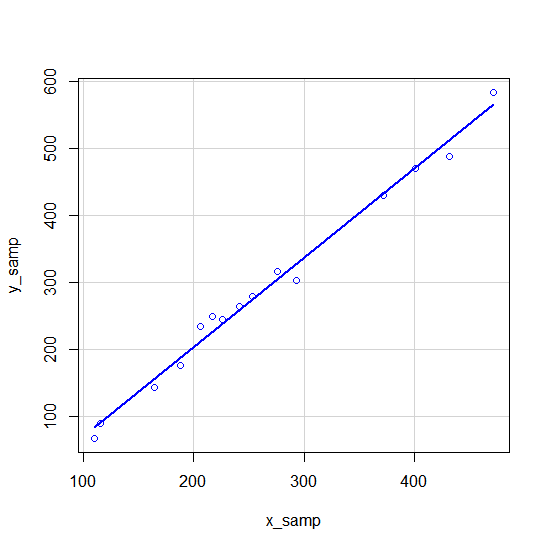
\includegraphics[width = .65\textwidth]{Rplot.png}
          \end{center}
        \end{figure}
        The data does look to be very linear, with constant variance. A ratio or regression estimator might work well. 
        \vspace{.15in}

        \item[b.] Use the regression estimation approach to estimate the true total value of all houses, $\tau_y$ with 
        a 95 percent confidence interval.\\
        \solution  Recall that $\tau_x = 512,400$ and that $N = 2000$ we get a $\mu_x = 512,400/2000$. Fitting a linear 
        model to the data in r, we get the following estimator, 
        \begin{equation*}
            \hat{\tau}_y = \beta_0 + \beta_1\tau_x = -63.717 +1.333(512,400)  = 682965.5
        \end{equation*}
        Using anova() we can quickly get the MSE them computing the variance we get, \\
        \textbf{Code:}
        \begin{center}
           \lstinputlisting{r1.txt}
        \end{center}
        \vspace{.15in}

        \item[c.] Use the usual SRS chapter 1 estimator using just the $Y$ values to get a 95 percent confidence interval.\\
        \solution First we compute the mean house value, then multiply it by the total number of houses $N = 2000$
        \begin{equation*}
            \hat{\tau}_{y} = \mu_yN = 288.6667(2000) =  577333.4
        \end{equation*}  
        Computing the variance an 95 percent confidence interval,\\
        \textbf{Code:}
        \begin{center}
           \lstinputlisting{r2.txt}
        \end{center}
        This estimator is considerably worse, the standard error is an order of magnitude greater which makes the confidence interval 
        a lot larger. The regression estimator uses information about $X$ and it's relation to $Y$ to reduce the variance, looking at the 
        SRS we can see how much that is leveraged to get a better estimator. 
    \end{enumerate}
\end{exercise}
\vspace{1in}




\begin{exercise}{2} Consider the following population, 
    \begin{equation*}
        \lbrace 1,2,3,2,4,5,7,6,5,8,10,12,12,13,12,14,15,14,16,16,13,15 \rbrace
    \end{equation*}
    \begin{enumerate}
        \item[a.] There are two possible 1-in-2 systematic samples. What are these? What is the
        probability that you will get the first of these samples?\\
        \solution The following is the sampling distribution for the population under  1-in-2 systematic sampling, 
   \begin{equation*}
        P(X = x) = \left\{\begin{array}{lr}
            \frac{1}{2} & $x = 1,3,4,7,5,10,12,12,15,16,13$ \\
            \frac{1}{2} & $x = 2,2,5,6,8,12,13,14,14,16,15$ 
            \end{array}\right\} 
   \end{equation*}
        
\vspace{.15in}


        \item[b.]   For each possible sample, compute the estimate of the population mean 
        $\mu$ and find its standard error (using the SRS formula we started with in this 
        class for the estimated mean and the standard error). 
        Is this estimator unbiased (how can you tell)? [Note: the 
        estimated mean from a systematic sample, using the SRS estimator, 
        CAN be slightly biased, if N isn’t an exact multiple of k.]\\
        \solution Computing the population mean for each sample we get, 
        \textbf{Code:}
        \begin{center}
           \lstinputlisting{r3.txt}
        \end{center}
        Systematic sampling experiences bias when the population is periodic, where the oscillations 
        match the sampling rate. Looking at our population we can see that we have an ordered population 
        which also results in bias in our standard error but it is biased low so we actually have higher accuracy than 
        what is reported. 
\vspace{.15in}

        \item[c.]  The SRS estimators of the standard error for each sample have been
         computed in part (b), so this is what you will actually see when you collect your
          sample (actually, you’ll only see one of them...). Do they seem to over-estimate 
          the actual variability of the sample means? How can you tell?\\
          \solution Like we illustrated before, since we have an ordered population we get a standard error which 
          is biased low. The estimator for the mean is unbiased, but our estimate of the standard error is larger than 
          the true standard error. 


    \end{enumerate}
\end{exercise}
\vspace{1in}






\begin{exercise}{3} Taking a close-to-systematic sample: Let’s say we have a frame 
    of $N = 100$ sampling units. We think there might be order in the values so we 
    would rather take a systematic sample rather than a SRS (WHY?), but we are afraid 
    of the bias that could occur in variance estimates for systematic samples if 
    there was periodicity in the population. \\

    Here is a way we can compromise. First, divide the frame into five strata each of
     size $N_i = 20$, with the first stratum consisting of the first 20 units in the
      frame, etc. Then take a SRS of size $n_i = 2$ from each stratum. This means
       you sample exactly 10 sampling units.\\
    \begin{enumerate}
        \item[a.]  Why is this less prone to problems with periodicity 
        (i.e. safer than a systematic sample) but less likely to have the 
        units clustered in one area in the population (as can happen in a SRS)?\\
        \solution This method has no set sampling rate, so it doesn't have the problem 
        of having the sampling rate match the periodicity of the data like you could have with one-in-k systematic 
        sampling. With the described sampling plan we also force the sample to have a good spread of the 
        population, sometimes a SRS will have bad spread. 
        \vspace{.15in}

        \item[b.]  Take a sample as described above from this population:
        \begin{equation*}
            pop <- c(8, 19, 31, 39, 51, 67, 54, 75, 87, 101, 103, 116, 107, 116, 
        113, 137, 148, 133, 150, 153, 165, 171, 161, 177, 209, 181, 231, 
        206, 212, 212, 237, 219, 222, 247, 229, 219, 238, 217, 216, 240, 
        276, 250, 247, 244, 259, 263, 249, 258, 226, 256, 250, 278, 243, 
        243, 240, 241, 230, 276, 238, 258, 236, 254, 223, 216, 230, 244,
         234, 232, 193, 197, 198, 206, 202, 188, 176, 191, 186, 158, 149, 
         152, 148, 130, 129, 136, 138, 134, 124, 89, 100, 93, 94, 76, 60, 
         56, 45, 30, 28, 10, 11, 10)
        \end{equation*} 
        Then compute a 95 percent confidence interval for the population mean $\mu$.\\
        \solution Sampling in r we get the following $\mu$ and confidence interval,\\
        \textbf{Code:}
        \begin{center}
           \lstinputlisting{r4.txt}
        \end{center}
        \vspace{.15in}

        \item[c.]   There is an attached paper (it uses Landsat data for a regression 
        estimator, but that’s not what I’m interested in at this point): Forest Area 
        Estimation Using Sample Surveys and Landsat MSS and TM data (F. Deppe, 1998), 
        Photogrammetric Engineering and Remote Sensing, vol. 64, No. 4, pp. 285-292). 
        Look at the part (including a figure) describing the Area Frame Sampling Scheme. 
        They treat it like a SRS as far as the estimate and standard error, but examine 
        Fig. 2, where it looks like they are taking a close-to-systematic sample. 
        Describe their sampling approach.\\
        \solution From what I could tell they used stratified sampling, but they split the population and sampled 
        the strata in a systematic way like what was described in the previous problem. First they split the 
        area of interest into 36 different strata. In each strata there were 49 different 1$km^2$ samples, and in each strata
        one sample was taken.


    \end{enumerate}
    \vspace{1in}
    
\end{exercise}

\begin{exercise}{4}  OK, systematic samples are... strange, though often very efficient.  
    For instance, the use of the usual sample average can lead to bias.  I'll show you 
    that with a very small population, then show you that there IS an unbiased estimator.  
    (This situation occurs when the population size isn't an exact multiple of $k$.)\\

    Consider this small population:  $\lbrace 1, 2, 3, 4, 10\rbrace$, with mean $\mu = 20/5 = 4$.  
    If we take a 1-in-2 sample, we get these two equally-likely samples:  $1, 3, 10$ and $2, 4$.\\
    \begin{enumerate}
        \item[a.] Compute the usual average (our unbiased estimator of $\mu$ when we used SRS) for each sample.  
        Since the samples are equally-likely, you can average the two averages to get $E(\overline{x})$.  
        Show that this isn't the same as the true population mean.  What does this tell you about the sample 
        average as an estimator of $\mu$ in this case?\\
        \solution From the following r analysis we can see that our systematic samples estimator for $\mu$ is not 
        an unbiased estimator since the expected value of the mean sampling distribution does not equal the population mean. \\
        \textbf{Code:}
        \begin{center}
           \lstinputlisting{r5.txt}
        \end{center}
        \vspace{.15in}



        \item[b.] There is a ... different... estimator of the population mean.  For each sample, you sum up the values, 
        multiply by the number of possible samples (2 in this case), then divide by the population size $N=5$.  
        In other words, $\hat{\mu} = {{k}\over{N}}\sum x_i$.  Compute this estimator for each sample.  Since the 
        two samples are equally-likely, the average of these two estimators is $E(\hat{\mu})$  Show that this 
        IS an unbiased estimator of the true population mean.  (This is based on a type of estimator that we'll 
        see later, called the Horvitz-Thompson estimator).\\
        \solution Performing the same analysis but with a new estimator, \\
        \textbf{Code:}
        \begin{center}
           \lstinputlisting{r6.txt}
        \end{center}
        \vspace{.15in}

    \end{enumerate}
    
    
\end{exercise}

\end{document}




















